\section{EVALUATION METHODOLOGY}\label{sec:expsetup}


\begin{figure}[!t]
	\centering
	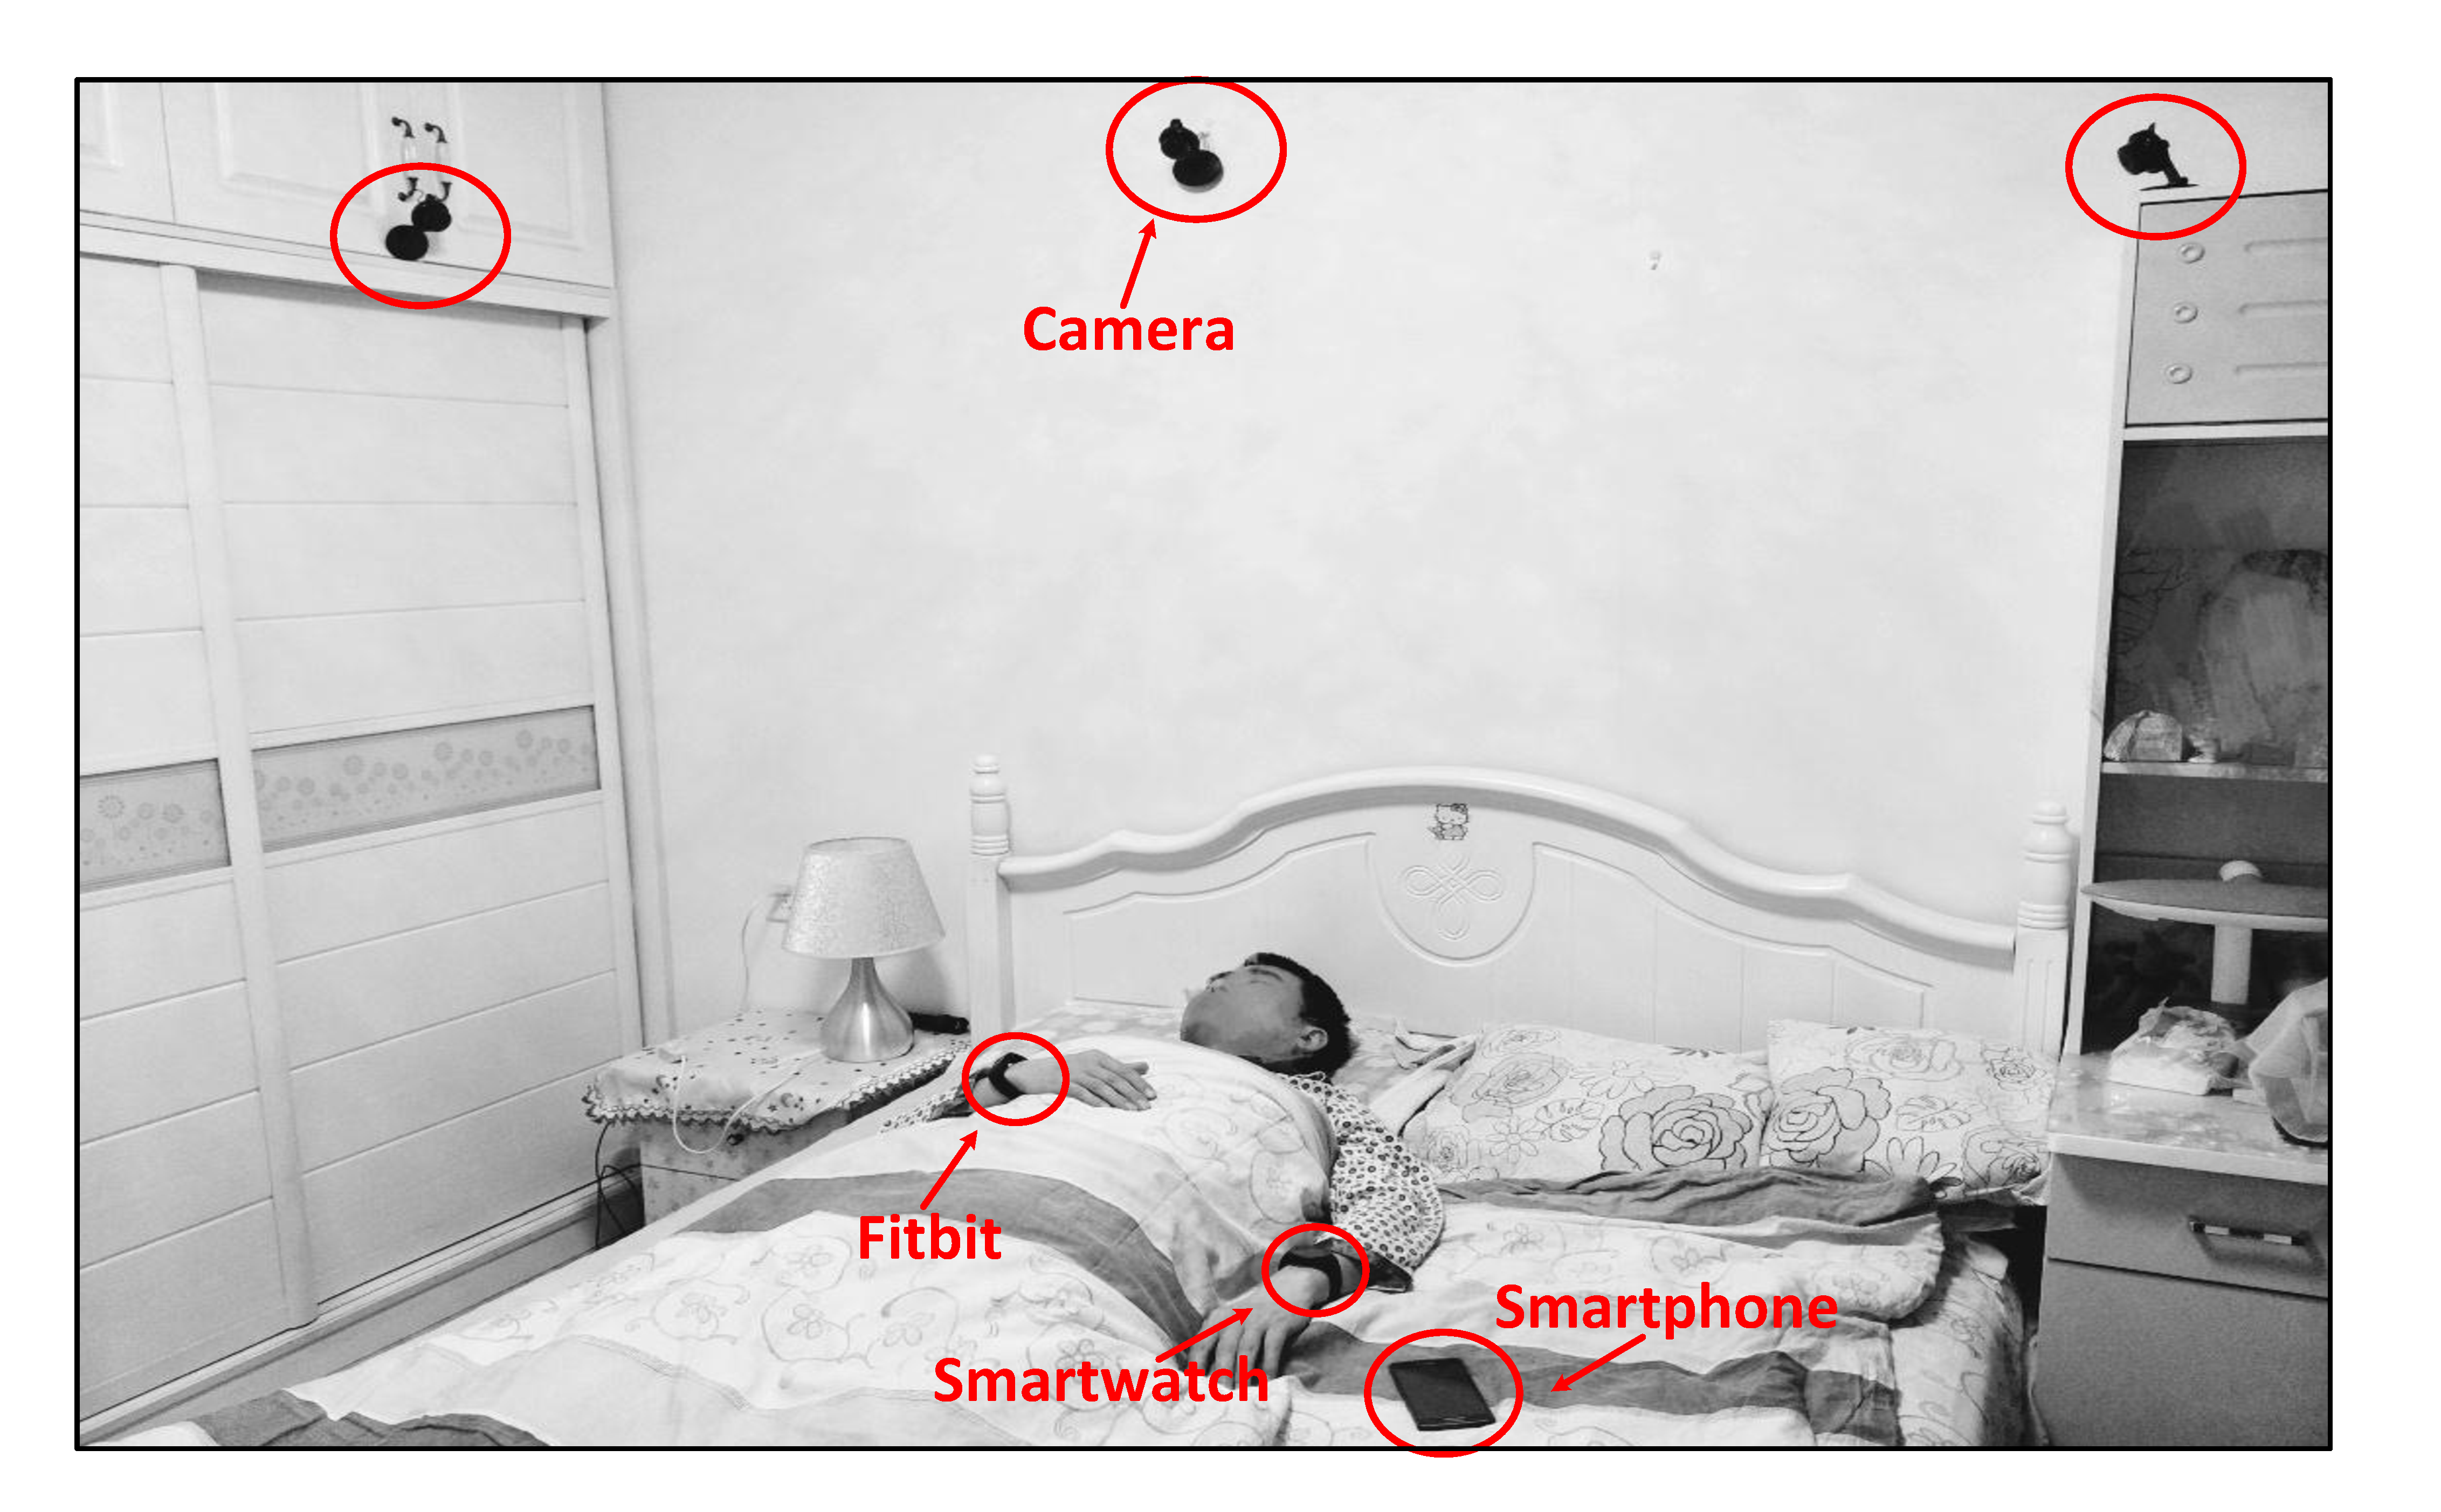
\includegraphics[width=0.57\linewidth]{Figures/setup.pdf}
	\caption{Experimental setup in one of our participants' home. }\label{fig:setup}
\end{figure}



\subsection{Experimental Setup\label{sec:evalusers}}

We evaluate {\systemname} through experiments conducted in $15$ single-occupancy homes over a two-week period.  The participants include 6 males and 9 females, whose age spans 15 to 60 years. To ensure too little sleep had no effect on the results, each participant was required to sleep at least $6$ hours per night during the study period. Two of our participants have been diagnosed with long-term, on-going sleep-related disorders, and one participant has described that his sleep is significantly affected by snoring. The remaining participants reported their sleep quality to go up and down. The study was approved by local IRB, and participants were separately asked to consent to release their data for analysis. In total, we collected 210 sets of nocturnal sleep data from our participants.

During the study, participants are asked to wear a smartwatch on their wrist. To obtain ground truth of sleep events, three video cameras were placed on the ceiling to monitor the user's sleep activities, as shown in Fig.~\ref{fig:setup}. The cameras have night vision and thus can capture sleep activity with high-quality. The video footage was manually labeled with different sleep activities and the labels were used as ground truth in our evaluation. Specifically, we consider the respiratory amplitude during the NREM stage as large amplitude, and the one during REM stage as normal amplitude. For the acquisition of sleep stage information, we confirm labels when both Fitbit and {\systemname} reach a consensus. To demonstrate the overall benefits of {\systemname} and the events captured by it, we separately collected ground truth information about sleep quality using questionnaires which were administrated each morning. The questionnaires were based on the Pittsburgh Sleep Quality Index (PSQI), a widely used and validated questionnaire in sleep quality research~\cite{buysse1989pittsburgh}. Finally, we collected sleep stage estimates from a Fitbit Charge2 and considered them as ground truth for sleep stage estimation. While the performance of Fitbit is not comparable to medical grade PSG, it has been shown to have a good association in adults~\cite{evenson2015systematic,fitbit01,fitbit02,fitbit03}, especially in estimating REM and light sleep stage. Equipping the participants with PSG was not feasible as it would disrupt their normal sleeping routines and potentially bias and reduce sleep activities, which are the main focus of our work. Moreover, the goal of our experiments is not to demonstrate that {\systemname} is capable of medical-grade sleep monitoring, but to demonstrate that it performs comparably to commercial systems in common sleep monitoring tasks, while at the same time being able to capture a much richer set of sleep information. We also compare our approach against Sleep Hunter~\cite{gu2016sleep}, a state-of-the-art mobile-based sleep monitoring approach, and a smartphone-based sleep monitoring app named Sleep as Android~\cite{SleepAndroid}. To provide a fair comparison against these baselines, we also place a smartphone next to the user's body on the bed to collect the data for Sleep Hunter and Sleep as Android.
	

\subsection{{Pilot Study: Training Data}}\label{sec:trainingdata}

Prior to our main study, we carried out a pilot study that was used to inform our algorithm design, and to provide training data for the algorithms integrated into {\systemname}. Our pilot study consisted of two groups (aged ranged from 15 to 60). One group   {consisted of} randomly selected 100 volunteers to conduct questionnaire surveys to provide the basis for our algorithm design. The other group consisted of 10 users whose data was used to train our models.


To improve the effectiveness of the algorithms integrated into {\systemname}, especially sleep posture and hand position detection, we elicited questionnaires to 100 volunteers to identify their common sleep posture. The main content of the questionnaire was about their common arm position in the four basic sleeping postures. Based on this investigation and previous research~\cite{position2014,HandPosition2}, we selected the positions to consider in {\systemname}. We also found that these arm positions are effective during the training and testing of the algorithm.

To train the models used in our system and to determine optimal parameter values, a small-scale pilot study with $10$ participants was carried out prior to the main experiment. The training examples used to train our algorithms and to determine the algorithm parameters are collected from 10 users (5 males and 5 females). Our testing users were asked to wear a smartwatch to sleep and collected the sensor data while they were sleeping. Every testing user contributes 10 nocturnal sleep data over a two-week period. These users were different from those taking part in our evaluation (Sec.~\ref{sec:evalusers}).



\subsection{Prototype Implementation \label{sec:implementation}}
We prototype and evaluate {\systemname} on a Huawei Smartwatch 2 wearable device. The smartwatch is equipped with a Quad-core Cortex-A7 processor at 1.1 GHz. It runs the Android Wear 2.0 operating system. We use five sensors of the smartwatch: the accelerometer, gyroscope, microphone, light sensor and orientation sensor. To reduce the energy consumption of the smartwatch, in the experiments we analyze the sensor data on a XiaoMI Note2 Android smartphone to which the smartwatch sends sensor measurements over Bluetooth. The sensors on the smartwatch are sampled every $30$ms, which was chosen to balance between information quality and energy consumption. {\systemname} starts tracking sleep events when it detects that the light is off and there has been nobody movement for 30 minutes. As part of an initialization process, {\systemname} estimates the initial body posture and hand position. It then uses these as a starting point to monitor sleep events like the body posture, rollovers, hand positions and body movements.
